\section{Data handling and design choices of the models}
This chapter presents how the pre-processed data is loaded and prepared for training of the models in Python, as well as the different architectures of the models, and features related to their implementation. Three separate model has been made fitting to each of the data representations presented in \ref{pre-processing}.  

\subsection{Data-handling in python}
The pre-processed data is loaded from a .mat file into python. 
Data within the file is pre-shuffled an split into a training and test subset, as described in \autoref{sec:pre-process}. 
The test subset will only be used to evaluate the generalization of the model, and therefore won't contain data that's been used during training \citep{Duda2000}. 
By keeping the test subset separate it will act as new unseen data, for the model. 
% The reason for shuffle the data is that improves generalisation through randomization. 
In Python the training subset is further split into a training and validation set. The validation set is used for estimating the generalization error of the model, and to examine how adjustments to hyperparameters effect the model \citep{Duda2000}.   
The validation set makes up 10\% of the available data for the different models. 



\subsection{Optimization techniques}
To try to reduce overfitting and improve generalization of the neural network different techniques are applied network models. 

One method known as grid search was used as to support the choice of some hyperparameters in the network. By using this method a listing of different hyperparameters can be tested on a model, that allows for choosing the parameter that gives the highest loss in validation error \citep{Goodfellow2016}.

Grid search is mainly practical when there are only a few hyperparameters that needs to be tested, because of the exponentially computational cost follows \citep{Goodfellow2016}.    


\subsubsection{Optimizer used for the models}
The Adam has been implemented in the three models, based on the findings written in \autoref{deeplearning}. 
BLA BLA I dont know what else to write.  

\subsubsection{Kernel-initializer 'Maybe'}
Kernel-initialization was performed, since this known to effect performance of the model. 
A grid search of kernel-initializer using uniform, lecun_uniform, normal, glorot_normal and glorot_uniform were tested and results revealed that glorot_normal performed the best by 3,2 \% compared to the second best. 
% See image kernal_init.png  


\subsubsection{Learning rate 'Maybe'}
In order to determine the most optimal Learning rate for the adam optimizer a several different learning rate were tested. 
A must because we have done this. 

IF WE CHOOSE ADAM IT'S IMPORTANT TO KNOW THAT IT ALREADY IS A OPTIMIZER WITH AN ADAPTIVE LEARNING RATE. 


\subsubsection{Manufacturing data 'Maybe'}
I don't think this is gonna be a reality 


\subsubsection{Batch training}
Initial experimentation of the batch size showed little flexibility, because of the available computation power for training of the model. The batch size could not exceed a value of four, as a result of the relative high image resolution (912 x 2315). As a result of this it was chosen reduce the resolution (233 x 251), by resizeing the images, as described in \ref{pre-prossesing}. 

Following grid search of batch parameters were performed with values of 5, 10, 15, 20, and the highest accuracy with the value of

ref to batch in deep learning section

 

 
 
\subsection{Training of the networks}
Supervised learning is used for training in all the models. The generic input for all of the model is gender, along with the different image representation, which are described in REF!!!. These inputs trained and then compared against their respective category label.   
The models classify data into three different classes e.g. duration interval of 0-12 months, 18-30 months and 36 months and above. Because of this multi classification, the output labels are changed from integer representation, 0 (0-12 months), 1 (16-30 months) and 2 ( and 36 months and above) into a one-hot encoded representation [0 , 0 , 1], [0 , 1 , 0] and [1 , 0 , 0] respectively. This is done by using keras utility function called \textit{to\_categorical}. 


\subsubsection{Cross-validation}
Because the amount of data for this project is limited it is chosen to implement m-fold cross validation, where the training data is divided into m number of subsets. Each of the subsets can function a either a validation set or as a part of a training set e.g. if a classifier is trained \textit{m} times, then each time a different subset will be used as a validation set, and the rest is used for training. \citep{Duda2000}
Because of the property of cross validation, it can be used as a way of investigate a general accuracy since all data is included during training, but may not be beneficial for every kind of problem. \citep{Duda2000}


\subsubsection{Dropout}
Dropout is a technique that can be used to prevent or reduce overfitting of a neural network. In a network the dropout can be applied to the individual layers, and works by randomly drop/”turn off” different nodes temporarily in the given layer during training. An illustration of the principle of dropout can be seen in \autoref{fig:Dropout}.  

\begin{figure} [H]
\centering
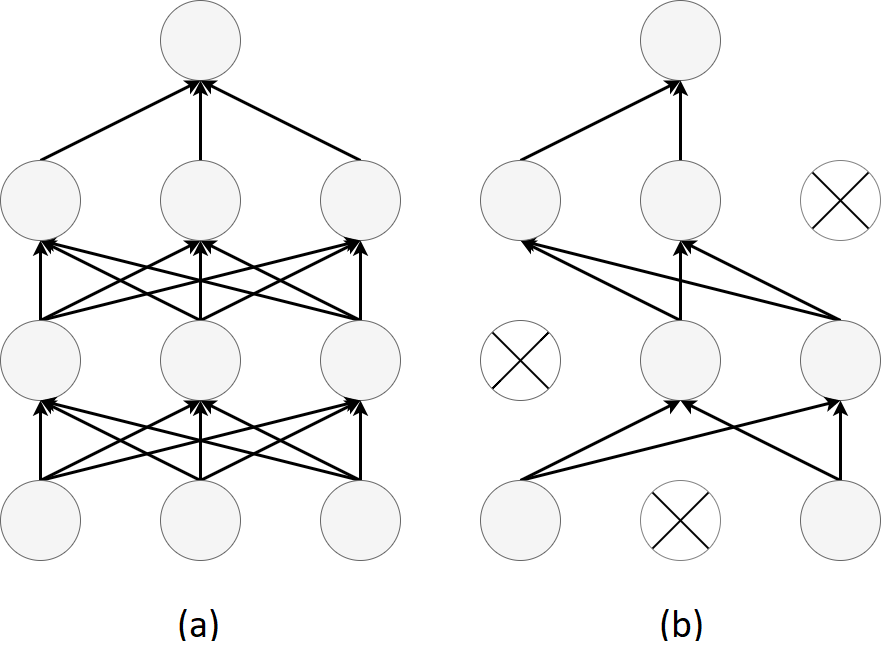
\includegraphics[width=0.6\textwidth]{figures/Dropout}
\caption{Illustration of dropout effect: The figure on the left illustrates a fully connected network, without dropout, and the right shows a network where dropout is enabled on the first three layers.}
\label{fig:Dropout}  
\end{figure}

This reduces co-adaptation, where nodes compute the same features, to where this may increase the generalisation capabilities for a neural network.\citep{Srivastava2014}  
A study, has tested the use of dropout in different neural networks, and indicates that the most optimal range of dropout is 20 \% of the nodes in the visible layers, and 50 \% in the hidden layers \citep{Srivastava2014}.
When implementing dropout to the models, it is defined in the given layers, and specified with a float value between 0 and 1, which defines the fraction of the nodes that drop \citep{Chollet2015}.







%Additional info that need to be placed somewhere. 
% There are simple methods that can be used to improve performance and training speed. Scaling of the input and giving an initial weight \citep{Duda2000}

For all the models the input and hidden layers uses the ReLu activation, since this is the most common used in neural network. \citep{Goodfellow2016} %Maybe the grid test suport ths as well, and maybe also something about computation power. 

and the sigmoid for the output layer.  




%TEMP CRAP THAT NEEDS TO BE PLACED ELSEWHERE
Temp-placehoder:
The process of making the neural network model has been a trial and error process, because there is not an actual “cookbook” for developing NN (This statement is from a not vaild source, but so far it’s the only one that i have found.) \citep{Goodfellow2016} 
